%========================================================================%
%               Copyright (C) 2016 All Rights Reserved.                  %
%             Author:BillHu<billhu@icloud.com>  Ver:<1.0>                %
%========================================================================%
%    The author grants permission, without fee and without a written     %
% license agreement, for use, reproduction, modification, and distribu-  %
% tion of this software and its documentation by educational, research,  %
% and non-profit entities for noncommercial purposes only.The above      %
% copyright notice and this paragraph MUST appear in all copies and      %
% modifications of the software and/or documentation.                    %
%========================================================================%
\documentclass{bjtuthesis}
%========================================================================%
% 自定义内容
%========================================================================%
\ctitle{中文题目}
\etitle{English Title}
\cauthor{作者}
\ctutor{导师}
\category{工学}
\major{土木工程}
\cid{14121023}
\jobtitle{教授}
\degree{硕士}
\field{桥梁工程}
\cdata{2017年3月}
%========================================================================%
% 自定义文字
%========================================================================%
\cthanks{放置在摘要页前,对象包括:1)国家科学基金,资助研究工作的奖学金基金,合同单位,资助或支持的企业、组织或个人。2)协助完成研究工作和提供便利条件的组织或个人。3)在研究工作中提出建议和提供帮助的人。4)给予转载和引用权的资料、图片、文献、研究思想和设想的所有者。5)其他应感谢的组织和个人。}
\cabstract{中文摘要应将学位论文的内容要点简短明了地表达出来,硕士学位论文一般为500~1000字,博士学位论文一般为1000~2000字。留学生英文版学位论文不少于3000字中文摘要,留学生英文版博士学位论文不少于5000字中文摘要。字体为宋体小四号。内容应包括工作目的、研究方法、成果和结论。要突出本论文的创新点,语言力求精炼。为了便于文献检索,应在本页下方另起一行注明论文的关键词(3-8个),如有可能,尽量采用《汉语主题词表》等词表提供的规范词。图X幅,表X个,参考文献X篇。}
\eabstract{Something Something Something Something Something Something Something Something Something Something Something Something Something Something Something Something Something Something Something Something.}
\cprelude{学位论文的序或前言,一般是作者或他人对本篇论文基本特征的简介,如说明研究工作缘起、背景、主旨、目的、意义、编写体例,以及资助、支持、协作经过等;也可以评述和对相关问题发表意见。这些内容也可以在正文引言中说明。}
%========================================================================%
% 前置部分
%========================================================================%
\begin{document}
\pagenumbering{roman}
\cover
\myclpage
\ccopyright
\myclpage
\setcounter{page}{1}
\ctitlepage
\myclpage
\thankspage
\myclpage
\cabspage
\myfanpage
\eabspage
\myfanpage
\cprepage
\myfanpage
\pagestyle{myfancy}
\tableofcontents
%========================================================================%
% 主体部份
%========================================================================%
\chapter{绪论}
\markboth{绪论}{}
\pagenumbering{arabic}
\setcounter{page}{1}
我是绪论。我是绪论。我是绪论。我是绪论。我是绪论。我是绪论。我是绪论。我是绪论。
\chapter{各种测试}
\section{图表测试}
\subsection{单张图片}
单张普通插图,及其引用,如图\ref{fig:G1}所示。

\begin{figure}[!htp]
\centering
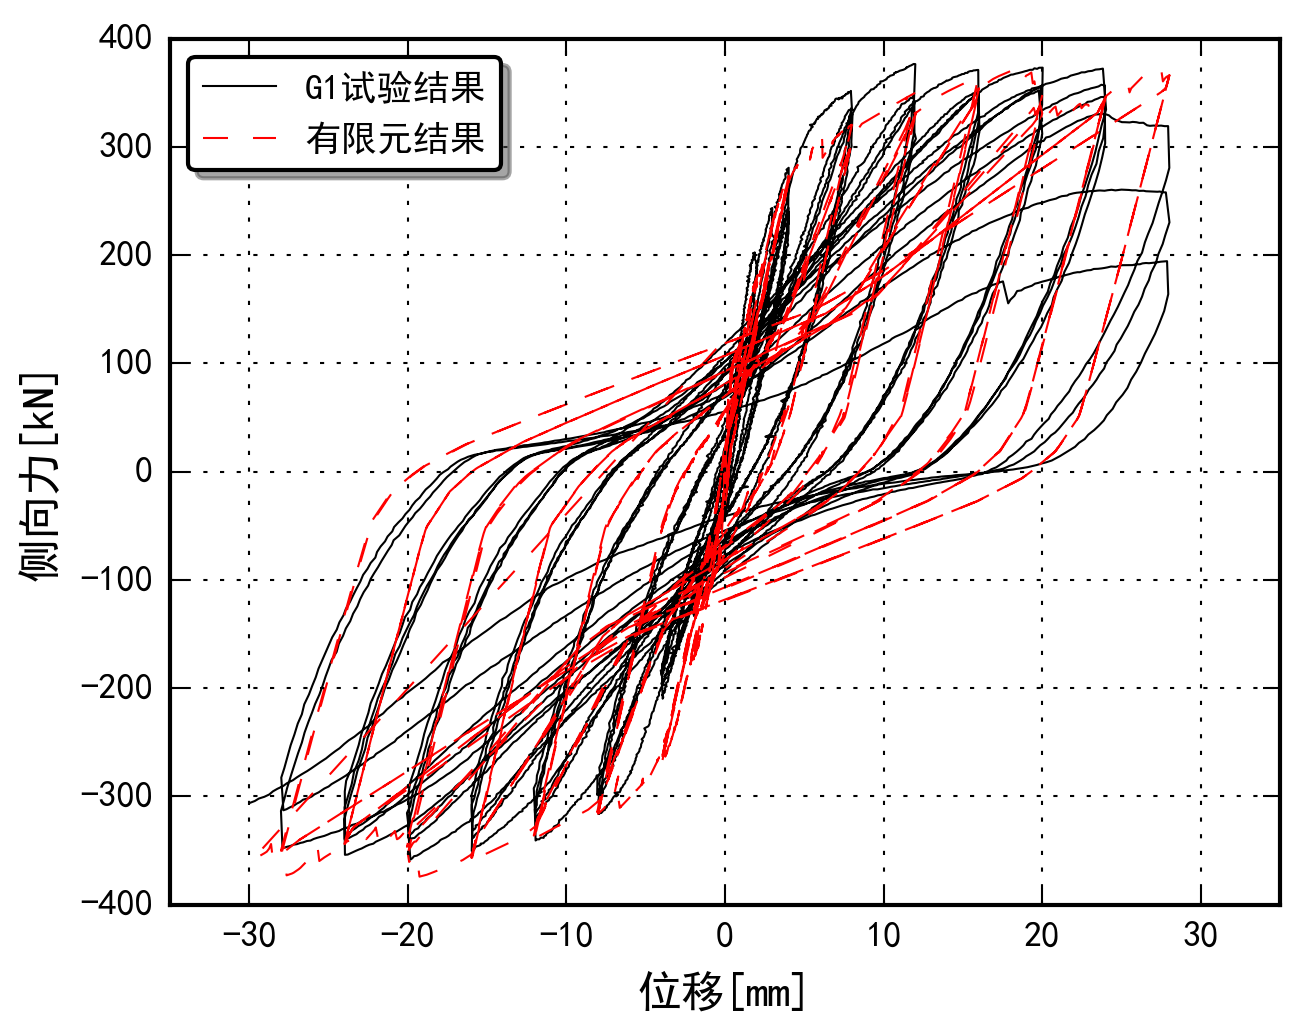
\includegraphics[width=0.8\textwidth]{pic/G1.png}
\figcaption{G1数据对比\label{fig:G1}}{Comparison of experimental data}
\end{figure}

\subsection{多张图片}
多张图片联排或者换行可以使用各种排版方式(minipage、subplot等),如下图\ref{fig:2}所示。
\begin{figure}
\centering
\begin{minipage}[t]{0.48\textwidth}
\centering
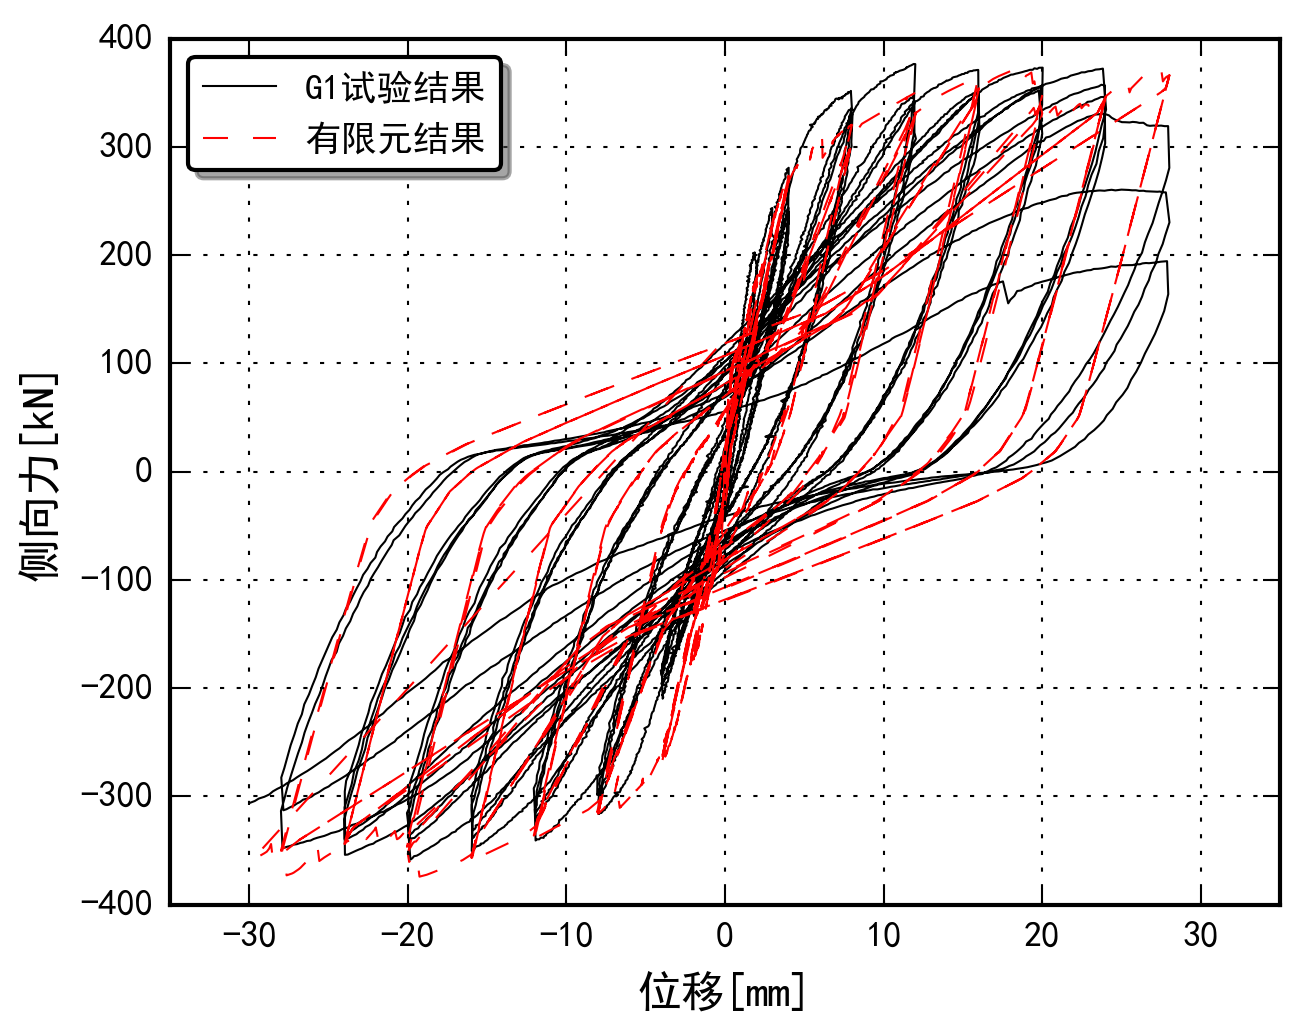
\includegraphics[width=0.9\textwidth]{pic/G1.png}\\
{\zihao{5}(a) G1试件}
\end{minipage}
\begin{minipage}[t]{0.48\textwidth}
\centering
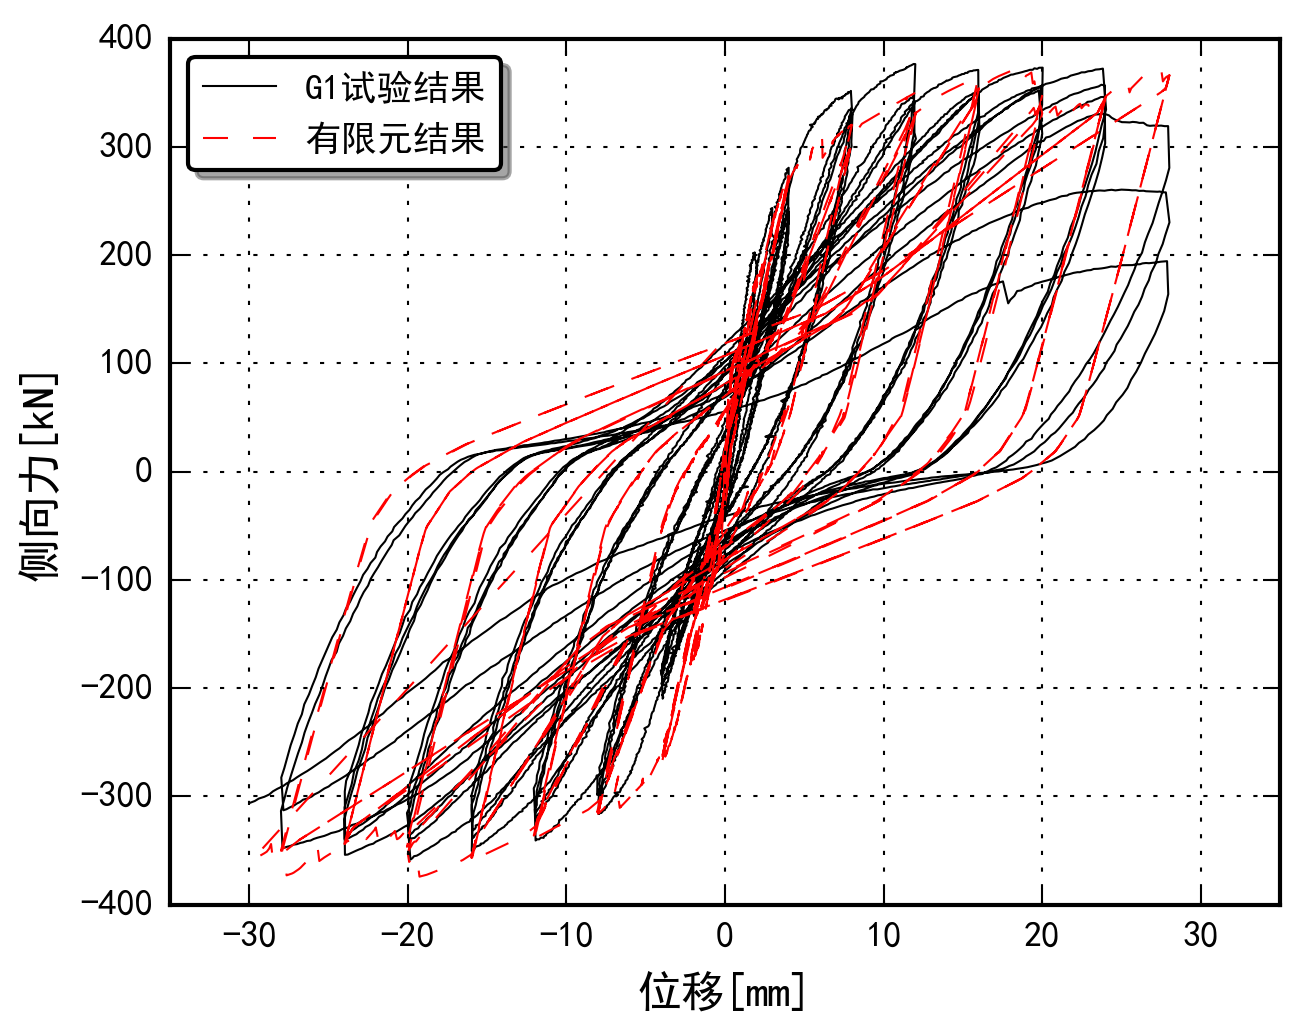
\includegraphics[width=0.9\textwidth]{pic/G1.png}\\
{\zihao{5}(b) G1试件}
\end{minipage}
\figcaption{G1数据对比\label{fig:2}}{Comparison of experimental data}
\end{figure}
\section{公式测试}
公式的排版和引用与正常\LaTeX\ 公式格式一致。例如:

\begin{equation}
\label{eqn:1}
e^{i\pi}+1=0
\end{equation}

欧拉公式(式\ref{eqn:1}),它是数学里最令人着迷的一个公式,它将数学里最重要的几个数学联系到了一起——两个超数:自然对数的底$e$,圆周率$\pi$;两个单位:虚数单位$i$和自然数的单位$1$,以及数学里常见的$0$。数学家们评价它是“上帝创造的公式”,我们只能看它而不能理解它。

\section{参考文献测试}
我使用的参考文献是符合《GB7714-2005》规范的中文论文参考文献格式。该规范作为国家标准化管理委员会正式公布的标准,其权威性和通用性远远超过了其它格式规范,是国内最正式的参考文献格式规范,并且是大多数高校毕业论文和杂志的指定参考文献格式。

下面分类测试各种类型参考文献:

\begin{itemize}
\item 中文规范\citep{C1}。
\item 英文规范\citep{ACI318}
\item 中文学位论文\citep{liguiqian}
\item 英文学位论文\citep{bentz2000}
\item 期刊\citep{FMK}
\item 图书类\citep{B1}
\item 其他\citep{R1}
\item 多文献引用,压缩格式\citep{C1,ACI318,liguiqian,R1}
\end{itemize}

\chapter{结论}
论文的结论是最终的、总体的结论,不是正文中各段的小结的简单重复。结论应该准确、完整、明确、精练。如果不可能导出应有的结论,也可以没有结论而进行必要的讨论。可以在结论或讨论中提出建议、研究设想、仪器设备改进意见以及尚待解决的问题等。
%========================================================================%
% 参考文献
%========================================================================%
\bibliography{MyDissBib}
\addcontentsline{toc}{part}{参考文献}
\cleardoublepage 
%========================================================================%
% 附录
%========================================================================%
\markboth{附录A}{}
\addcontentsline{toc}{part}{附录A}
\begin{center}
{\zihao{3}\heiti 附录A}
\end{center}
\begin{center}
{\zihao{3}\heiti 附录标题}
\end{center}

\indent\zihao{5}附录是作为论文主体的补充项目,并不是必须的。
论文的附录依序用大写正体英文字母A、B、C……编序号,如:附录A。
\cleardoublepage
%========================================================================%
% 索引
%========================================================================%
\markboth{索引}{}
\addcontentsline{toc}{part}{索引}
\begin{center}
{\zihao{3}\heiti 索引}
\end{center}

\indent\zihao{5}按照需要编排分类索引、著者索引、关键词索引等。
\cleardoublepage
%========================================================================%
% 作者简历及研究成果
%========================================================================%
\markboth{作者简历及攻读硕士学位期间取得的研究成果}{}
\addcontentsline{toc}{part}{作者简历及攻读硕士学位期间取得的研究成果}
\begin{thecenter}
作者简历及攻读硕士学位期间取得的研究成果
\end{thecenter}

\zihao{5}包括教育经历、工作经历、攻读学位期间发表的论文和完成的工作等。行距16磅,段前后各为0磅。
\cleardoublepage
\cstatement
\clastpage
\end{document}
